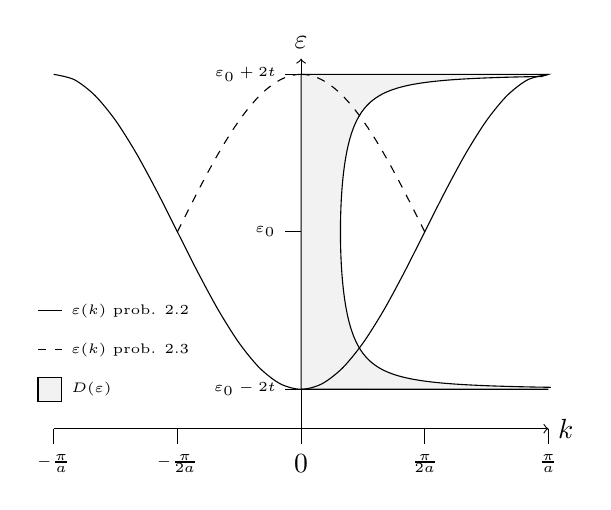
\begin{tikzpicture}
    % Axes
    \draw[->] (-pi,0) -- (pi,0) node[right] {$k$};
    \draw[->] (0,-0.2) -- (0,4.7) node[above] {$\varepsilon$};
    
    % Ticks
        %y
        \draw (0,4.5) -- (-0.2,4.5) node[left] {\tiny{$\varepsilon_0 + 2t$}};
        \draw (0,2.5) -- (-0.2,2.5) node[left] {\tiny{$\varepsilon_0$}};
        \draw (0,0.5) -- (-0.2,0.5) node[left] {\tiny{$\varepsilon_0 - 2t$}};
        
        %x
        \draw (-pi,0)   -- (-pi,-0.2)    node[below] {\tiny{$-\frac{\pi}{a}$}};
        \draw (-pi/2,0) -- (-pi/2,-0.2)  node[below] {\tiny{$-\frac{\pi}{2a}$}};
        \draw (0,0)     -- (-0,-0.2)     node[below] {$0$};
        \draw (pi/2,0)  -- (pi/2,-0.2)   node[below] {\tiny{$\frac{\pi}{2a}$}};
        \draw (pi,0)    -- (pi,-0.2)     node[below] {\tiny{$\frac{\pi}{a}$}};
    
    % Legend
    \draw (-pi-0.2,1.5) -- (-pi+0.1,1.5) node[right] {\tiny{$\varepsilon(k)$ prob. 2.2}};
    \draw[dashed] (-pi-0.2,1) -- (-pi+0.1,1) node[right] {\tiny{$\varepsilon(k)$  prob. 2.3}};
    \draw (-pi-0.2,0.5) -- (-pi+0.1,0.5) node[right] {\tiny{$D(\varepsilon)$}};
    \filldraw[fill=black!5!white] (-pi-0.2,0.35) rectangle (-pi+0.1,0.65);
    
    % DOS
    \filldraw[color=black,fill=black!5!white,smooth,samples=1000,variable=\y,domain=0.525:4.475] (0,0.5) -- (pi,0.5) plot ({(1/2)/(sqrt(1-(\y-2.5)*(\y-2.5)/4))},{\y}) --(pi,4.5) -- (0,4.5) -- (0,0.5);
    
    % Bands
    \draw[color=black,smooth,domain=-pi:pi]  plot (\x,{2.5-2*cos(\x r)});
    \draw[color=black,dashed,smooth,domain=-pi:(-pi/2)]  plot (\x+pi,{2.5-2*cos(\x r)});
    \draw[color=black,dashed,smooth,domain=(pi/2):pi]  plot (\x-pi,{2.5-2*cos(\x r)});
\end{tikzpicture}
